\section{Experiments}
\label{sec:experiments}
The research problems we want to tackle here are: 
(1) Can KPCNet generate more specific CQs? 
(2) To what extent can we control the generation of KPCNet by operating on the keywords? 
(3) How well can our proposed keyword selection methods promote local diversity, compared to existing diverse generation approaches?

\subsection{Evaluation metrics}
Most previous works on question generation \citep{jain2017creativity, hu2018aspect, rao2019answer} adopts \textit{Individual-level} evaluation protocol, where only the best generated question of a group is evaluated (thus also named \textit{Oracle} metrics). Specially, to deal with our last research problem, we need to evaluate the diversity within a generation group. We refer to this as \textit{Group-level} evaluation. We evaluate with automatic metrics as well as human judgements on both level. 

\subsubsection{Automatic Metrics}
Following \citep{rao2019answer}, We use \textbf{Distinct-3} (DIVERSITY), \textbf{BLEU}\footnote{\url{https://github.com/moses-smt/mosesdecoder/blob/master/scripts/generic/multi-bleu.perl}}\citep{papineni2002bleu} and 
\textbf{METEOR} \citep{banerjee2005meteor} for individual-level automatic evaluation.

For group-level evaluation, we adopt the evaluation protocol proposed by \citet{shen2019mixture} for diverse machine translation, and use \textbf{Pairwise-BLEU} and \textbf{Avg BLEU} as the evaluation metric.

\subsubsection{Human Judgements}
% \KZ{How many annotators? What about inter-judge agreement? Computer kappa agreement.}
% \Zl{Actually, I myself is the only annotator. So there's no inter-annotator agreement at all.}
For individual-level human judgements, we show the annotator one context and one generated question for each system (including reference). The system name is invisible to the annotator and the order is randomly shuffled. The selected candidate is the one that achieved the highest BLEU in the generation group. 

Inspired by \citet{rao2019answer}, we ask human to judge the \textbf{Grammaticality(G), Relevance(R), Seeking New Information(N) and Specificity(S)} of the questions. Also, noting that the system generations are also prone to make logical errors like improper repetition (``does the lid have a lid ?") or asking for relevant but not exactly the correct object (asking ``what is the thickness of the bed ?" for a mattress), we further judge the \textbf{Logicality(L)} of the candidate.

For group-level human judgements, we run the deduplication procedure (Sec \ref{sec:deduplicate}) to get 3 top questions for each system. And annotators are showed one context and the selected 3 questions for every group. The groups are also anonymized and shuffled.

For each question in a group, we score the same metrics as those for individual-level judgements. To evaluate the valid variety of each group produced by local generation diversity, we introduced an additional and important group-specific metric: \textbf{\#Useful}. This is the number of useful questions after excluding problematic (ungrammatical, irrelevant, illogical, etc.) and semantically equivalent questions within a group. And we further calculate \textbf{\#Redundant} as (the number of unproblematic questions - \textbf{\#Useful}) to measure local redundancy.

Individual-level and group-level evaluation was conducted on the same set of 100 sample products.

\subsection{Dataset}
We evaluate our model on the \texttt{Home \& Kitchen} category of the Amazon Dataset preprocessed by \citet{rao2019answer}. We applied extra preprocessing on the raw data to remove noises in dataset (Appendix A). In this dataset, \textit{context} is the product title concatenated with the product description, and \textit{question} is the CQ asked by customers to the product. It consists of 19,119 training, 2,435 validation and 2,305 test examples (product descriptions), with 3 to 10 questions (average: 7) per description. The inherent diversity of questions in the dataset allows the proper evaluation of group-level generation diversity. We processed another category, \texttt{Office}, in a similar way. This is a much smaller dataset, consisting of 2,190 training, 285 validation and 256 test examples, with 3 to 10 questions (average: 6) per description. We will first analyze the results on \texttt{Home \& Kitchen} in detail, then briefly discuss the results on \texttt{Office}.

\subsection{Baselines}

For individual-level generation, we compare KPCNet with the following models: \textbf{MLE} Vanilla seq2seq model trained on (context, question) pairs using maximum likelihood objective.  \textbf{hMup} A representative of the family of mixture models proposed in \citet{shen2019mixture}, which achieved a good balance of overall quality and diversity.\footnote{We also tried GAN-Utility \citep{rao2019answer}, but failed to reproduce a plausible result possibly due to the instability of GAN training.}

For a fair comparison, we control the encoder and decoder for all the above methods to have a similar 2-layer GRU \citep{cho2014learning} or LSTM \citep{hochreiter1997long} architecture and close amount of parameters. 

For group-level generation, we compare across 3 categories of diverse generation methods:

\paragraph{Decoding based} Classical beam search naturally produces different generation on each beam. Therefore, we evaluate the effect of beam search combined with MLE and KPCNet with threshold selection [KPCNet(beam)]. Recently, several decoding approaches \citep{ippolito2019comparison} are proposed to further promote diversity in generation, and \textit{Diverse Beam Search}\citep{vijayakumar2018diverse} is one of the representative methods. So we also evaluate KPCNet with diverse beam search [KPCNet(divbeam)].

\paragraph{Model based} hMup is designed for diversity at the model level. It provides a discrete latent variable called \textit{expert} to control the generation. We thus take the top beam-searched candidate of each expert to form a generation group for evaluation.

\paragraph{Keywords based} This is dedicated to KPCNet. We evaluate the \textit{Sampling}[KPCNet(sample)] and \textit{Clustering}[KPCNet(cluster)] methods for keyword selection. We also investigate the potential of KPCNet with knowledge (Sec \ref{sec:knowledge}) by providing the ground truth keyword set [KPCNet(truth)].

All systems using beam search have a beam size of 6, we also set number of experts for hMup to 6, and we use beam size of 6 with 3 diverse groups for \textit{diverse beam search}. We select 2 keyword groups for KPCNet(sample) and KPCNet(cluster). To produce the final generation group for evaluation, outputs of all systems will go through the same deduplication postprocessing (Sec \ref{sec:deduplicate}) to get 3 questions for each group.

\subsection{\texttt{Home \& Kitchen} Dataset Results}

\subsubsection{Individual-level Evaluation}

Table \ref{tab:ind-auto-eval} shows the automatic evaluation results. KPCNet and hMup outperform MLE in METEOR but not in BLEU. We claim that it is due to the shorter and the safer generation of MLE, which is naturally favored by precision-based BLEU but not F-based METEOR. The average generation length is 5.957 for MLE, 8.231 for hMup, and 7.263 for KPCNet. KPCNet significantly outperform all the other baselines in Distinct-3 and METEOR, showing that KPCNet potentially promote higher global diversity and generation quality. We note that KPCNet(truth) has a great advantage over KPCNet, indicating the controllability of keywords and the potential of KPCNet to be further strengthened by improving the conditioned keyword set with other helpers like external knowledge (Sec \ref{sec:knowledge}).

\begin{table}[h]
  \small
  \centering
  \begin{tabular}{l|ccccc}
  \hline
  {} & Distinct-3 & BLEU & METEOR \\
  \hline
  ref  &        0.6934 &        - &    - \\
  \hline
  MLE &        0.0777 &  \textbf{18.13} & 14.86 \\
  hMup &        0.1111 &  17.76 &    15.40  \\
  KPCNet &        \textbf{0.1530} &     17.77 &    \textbf{16.18}  \\
  \hline
  KPCNet(truth) &        0.3738 &     23.63 &    19.38  \\
  \hline
  \end{tabular}
  \caption{\label{tab:ind-auto-eval} Individual-level automatic evaluation results on \texttt{Home \& Kitchen} dataset.}
\end{table}

\begin{table}[bp]
  \small
  \centering
  \begin{tabular}{l|ccccc}
  \hline
  {} & G & R & L & N & S \\
  \hline
  ref  &        0.98 &        1.00 &    1.00 &     0.94 &     2.68 \\
  \hline
  MLE  &        \textbf{0.99} &     0.92 &    \textbf{0.98} &     \textbf{0.85} &     1.45 \\
  hMup &        \textbf{0.99} &     0.92 &    0.86 &     0.81 &     1.81 \\
  KPCNet &        \textbf{0.99} &     \textbf{0.99} &    0.95 &     0.80 &     1.81 \\
  KPCNet(filter) &        \textbf{0.99} &     \textbf{0.99} &    0.94 &     \textbf{0.85} &     \textbf{1.84} \\
  \hline
  \end{tabular}
  \caption{\label{tab:ind-human-eval} Individual-level human evaluation metrics on 100 sample products from \texttt{Home \& Kitchen}. G/R/L/N/S stand for Grammatical, Relevance, Logicality, New Info and Specificity respectively.}
\end{table}


\begin{table*}[htbp]
  \centering
  \small
  \begin{tabular}{l|ccccccc}
    \hline
    {} & Relevant\tiny{[0-1]} & Logical\tiny{[0-1]} & New Info\tiny{[0-1]} & Specific\tiny{[0-4]} & \#Useful\tiny{[0-3]} & \#Redundant\tiny{[0-2]} & Avg Rank \\
    \hline
    ref          &    0.990 &   1.000 &    0.947 &    2.530 &   2.680 &      0.120 & - \\
    \hline
    MLE          &    0.907 &   \textbf{0.943} &    \textbf{0.863} &    1.457 &   1.550 &      0.590 & 3.667 \\
    hMup         &    0.900 &   0.793 &    0.833 &    1.727 &   1.530 &     \textbf{0.130} & 4.667 \\
    \hline
    KPCNet(-filter)  &    \underline{\textbf{0.987}} &   \underline{0.870} &    \underline{0.830} &    1.757 &   1.280 &      0.750 & 4.500 \\
    KPCNet(beam)    &    \underline{\textbf{0.987}} &   \underline{0.853} &    \underline{\textbf{0.863}} &    1.793 &   1.330 &      0.750 & 3.667 \\
    KPCNet(divbeam) &    \underline{0.963} &   0.780 &    \underline{0.860} &    1.760 &   1.480 &  \underline{0.310} & 4.167 \\
    KPCNet(sample)  &    \underline{0.963} &   \underline{0.837} &    \underline{0.850} &    \underline{\textbf{1.890}} &   1.500 &      0.450 & 3.500 \\
    KPCNet(cluster)  &    \underline{0.963} &   \underline{0.863} &    \underline{0.823} &    \underline{1.877} &   \underline{\textbf{1.760}} &      \underline{0.190} & \textbf{3.000} \\
    \hline
    \end{tabular}
  \caption{\label{tab:group-human-eval} Group-level human evaluation results on 100 sample products from \texttt{Home \& Kitchen}. Grammatical is omitted as the results are similar to Table \ref{tab:ind-human-eval} where all systems performs well. \textit{Avg Rank} is the average ranking among all 7 methods across the 6 metrics. We perform hypothesis test among KPCNet variants, and the difference between underlined and non-underlined numbers at each column is statistically significant with $p \leq 0.05$.}
  \end{table*}

  % \KZ{The human eval results seem random. Can we reach some conclusion?}
Table \ref{tab:ind-human-eval} shows the individual-level human evaluation results. We can see that all systems perform well in \textit{Grammatical}, KPCNet significantly outperform other systems in \textit{Relevant} and achieved the best \textit{Specific}, while perform slightly worse in \textit{Logical}. The superior \textit{Relevant} proves our hypothesis that independently trained keyword predictor help focus on relevant keywords instead of irrelevant but generic words preferred by MLE (Sec \ref{sec:specific}). KPCNet(filter) gets a much higher \textit{New Info} at the cost of only slight drop in \textit{Logical}. This shows that the Keyword Filtering trick (Sec \ref{para:filter}) can truly utilize the controllability of keywords to help avoid repetition. Therefore, we by default incorporate the trick with all the KPCNet variants in the next group-level evaluation stage while keep the plain KPCNet for comparison as KPCNet(-filter).

\subsubsection{Group-level Evaluation}

  \begin{figure}[htbp]
    \centering
    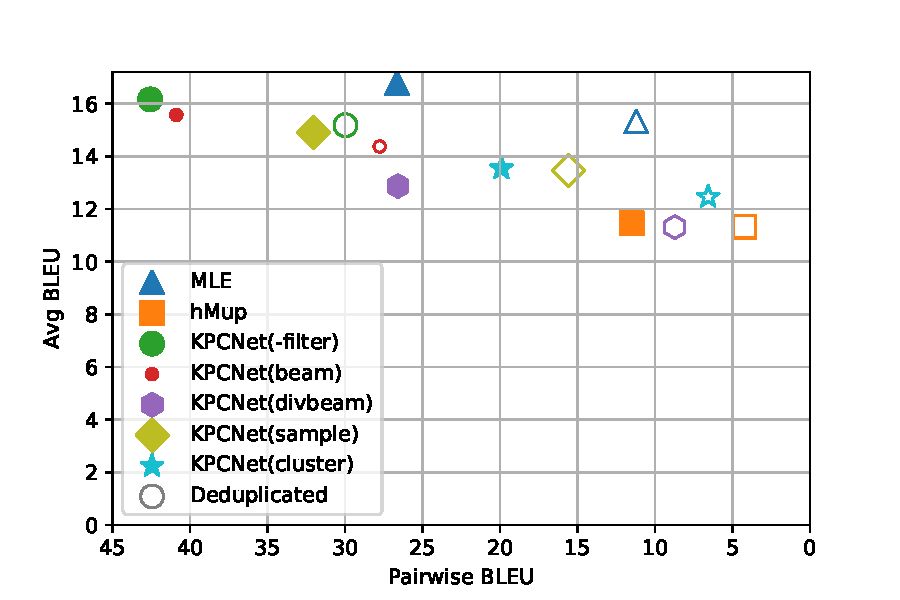
\includegraphics[width=\linewidth]{tradeoff-2BLEU.pdf}
    \caption{Group-level Automatic metrics on the whole test set of \texttt{Home \& Kitchen}. The lower Pairwise BLEU, the more diverse for the generation group. Solid markers are the results for the top 3 candidates in the original group, while hollow markers measures the remaining 3 after deduplication (Sec \ref{sec:deduplicate}).}
    \label{fig:group-filter}
    \end{figure}


The group-level automatic evaluation metrics before and after deduplication  (Sec \ref{sec:deduplicate}) for each system is shown in Figure \ref{fig:group-filter}. Original results (solid markers) showed that hMup has the highest local diversity while has the poorest Avg BLEU. MLE has moderate level of local diversity and the highest Avg BLEU, and we found that Keyword Filtering slightly harmed Avg BLEU, which is against our intuition. But we later found Avg BLEU doesn't correlate well with most human judgements (Appendix B). Several diversity-promoting variants of KPCNet improved local diversity at the cost of Avg BLEU, among which KPCNet(cluster) achieved a best tradeoff between the two. Comparing the original and deduplicated results (hollow markers), we can see that our simple heuristic can effectively eliminate redundancy at the cost of slight degradation of Avg BLEU, as only nearly identical hypotheses with high BLEU are excluded. 

Group-level human evaluation results are shown in Table \ref{tab:group-human-eval}. We can see that all KPCNet variants clearly outperform baselines in \textit{Relevant} and \textit{Specific} while have a competitive performance in \textit{New info}. MLE rated best for \textit{Logical} for its conservative generations (low \textit{Specific}), and the questions tend to overlap with each other, as is reflected in high \textit{\#Redundant}. KPCNet(beam) has a even higher redundancy since its searching space is further limited by the conditioned keyword set. Diverse generation variants can help overcome this drawback. Especially, KPCNet(cluster) achieved the best \textit{\#Useful}, \textit{Avg Rank}, and its performance on all metrics is among the best of KPCNet variants. This shows that the semantically-coherent keyword sets produced by clustering can effectively improve the generation diversity and quality of KPCNet. 

\subsubsection{Case Study}
\begin{table}[h]
  \small
  \centering
  \begin{tabular}{l|l}
  \hline
  Product & \makecell[l]{Novaform memory foam comfort curve pillow} \\
  \hline
  \makecell[l]{KPCNet \\ (cluster)} & \makecell[l]{is this a \textbf{firm} \textbf{pillow}? (pillow, foam, sleep, firm) \\ is this pillow good for \textbf{stomach sleepers}? \\ (stomach, sleeper)} \\
  \hline
  Product & \makecell[l]{full-sized headboard in solid wood} \\
  \hline
  \makecell[l]{KPCNet \\ (cluster)} & \makecell[l]{what is the height of this \textbf{headboard} ? \\ (bed frame headboard) \\ does it have a \textbf{box spring} ? (mattress box spring)} \\
  \hline
  \end{tabular}
  \caption{\label{tab:kwd-cluster} Example generation groups for KPCNet(cluster). Keywords in the parentheses.}
  \end{table}

  

\begin{table*}[htbp]
  \centering
  \small
  \begin{tabular}{l|ccccccc}
  \hline
  {} & Grammatical\tiny{[0-1]} & Relevant\tiny{[0-1]} & Logical\tiny{[0-1]} & New Info\tiny{[0-1]} & Specific\tiny{[0-4]} & \#Useful\tiny{[0-3]} & \#Redundant\tiny{[0-2]} \\
  \hline
  ref         &       0.993 &    0.997 &   0.993 &    0.933 &    2.713 &   2.420 &      0.330 \\
  \hline
  MLE         &       0.970 &    0.843 &   \textbf{0.883} &    0.797 &    1.470 &   1.070 &      0.420 \\
  KPCNet &       \textbf{0.993} &    \textbf{0.940} &   0.817 &    \textbf{0.803} &    \textbf{1.903} &   \textbf{1.470} &      \textbf{0.190} \\
  \hline
  \end{tabular}
  \caption{\label{tab:group-human-eval-office} Group-level human judgments on 100 samples from the \texttt{Office} dataset. KPCNet here uses keyword clustering.}
\end{table*}


Table \ref{tab:kwd-cluster} provided 2 example generation groups of KPCNet(cluster). For each group, the 6 predicted keywords captured specific aspects of the product. Then they are divided into 2 coherent groups (as they formed natural phrases such as ``firm pillow'' and ``stomach sleeper'') by clustering. Finally, the different conditioned keyword sets are reflected in the generation. In the first case, specific and diverse generations are successfully produced with precisely predicted keywords. However, the second question in another case is illogical. The possible reason is that keyword predictor produced related but unsuitable keywords ``box spring'', which can be asked for a whole bed but not for headboard alone. This shows that predictor is the performance bottleneck of KPCNet. We provide an example of group-level human judgement results including all systems in Appendix B.

\subsection{\texttt{Office} Dataset Results}


\begin{table}[h]
  \centering
  \small
  \begin{tabular}{l|ccccc}
  \hline
  {} & Distinct-3 & BLEU & METEOR \\
  \hline
  ref  &        0.7554 &        - &    - \\
  \hline
  MLE &        0.2033 &  \textbf{14.73} & 13.81 \\
  hMup &        0.1531 &  10.45 &    12.52  \\
  KPCNet &        \textbf{0.3099} &     13.84 &    \textbf{15.29}  \\
  \hline
  \end{tabular}
  \caption{\label{tab:ind-auto-eval-office} Individual-level automatic evaluation results on the \texttt{Office} dataset.}
\end{table}

For brevity, we only show the individual-level automatic evaluation and group-level human judgement results. All the experimental settings are the same with the previous experiments, except that we apply no keyword filtering here. 

Table \ref{tab:ind-auto-eval-office} showed that KPCNet still outperforms MLE in Distinct-3 and METEOR, while falls behind at BLEU. Both the automatic metrics and our manual check indicate that hMup fails to give comparable performance at the small dataset, so we exclude it in group-level evaluation. 

Table \ref{tab:group-human-eval-office} showed that the performance of both models degraded here possibly due to the smaller data size. However, the observation is similar. KPCNet(cluster) outperforms MLE in most metrics especially at \textit{Relevant}, \textit{Specific} and \textit{\#Useful} despite a weakness at \textit{Logical}. This shows that KPCNet(cluster) can consistently improve the diversity and specificity of the generation.

